% Latest version available here:  https://github.com/LIKS/phd_report_template_en
% Any suggestions or contributions are welcome!  Also see: http://latex.liks.lt!
\documentclass[11pt, a4paper]{article}
\usepackage[utf8]{inputenc}
\def\LTfontencoding{L7x}
\usepackage[\LTfontencoding]{fontenc}
\usepackage[english]{babel}
\usepackage{PhDReportEN}
\usepackage{amsmath}
\usepackage{bm}
\usepackage{amsfonts}
\usepackage{float}
\usepackage{graphicx}
\usepackage{color}
\usepackage{listings}
\usepackage{wrapfig}
\usepackage{algpseudocode}
\usepackage{algorithm}
\usepackage{algorithmicx}
\usepackage{caption}
\usepackage{subfig}
\usepackage{datetime}
\usepackage{cite}

\universitytitle{Vilnius University}
\departmenttitle{Institute of Mathematics and Informatics}
\departmentdetails{VU Institute of Mathematics and Informatics, Akademijos str.
4, Vilnius LT-08663, \\ Lithuania \\ \href{http://www.mii.lt}{www.mii.lt}}
\universitylogo{img/vu_logo}
\departmentlogo{img/mii_logo}
\date{\monthname\ \the\year}
\scientifictrend{Informatics (09 P)}
\reportid{MII-DS-09P-\shortyear-<report nr.>}

\title{<Thesis title>}
\author{<Author>}

\begin{document}

\maketitle

\sectionnonumnocontent{Abstract}
.........

\keywords{.........}

\tableofcontents

\section{Introduction}

\section{<main part of the report >}
The report should contain material, which the author was committed to prepare
for the reporting period (write a thesis section, create some kind of
methodology etc.; texts of papers ready for publishing can be included).
Preparation of the report is optional if the author did not have this kind of
commitments.

\section{Conclusions}

\section*{\emph{References}}% If you use \cite at least once, comment this line;
                            % Uncomment the next line and lines in Makefile. 
% \bibliography{bibliografija}   

\appendix
\section{Algorithm experimental comparison results}
% tablesgenerator.com - converts calculators, e.g. excel, tables to LaTeX
\begin{table}[H]
  \centering
  \caption{Table example.}
  {\begin{tabular}{|l|c|c|} \hline
    Algorithm    & $\bar{x}$ & $\sigma^{2}$ \\
    \hline
    Algorithm A  & 1.6335    & 0.5584       \\
    Algorithm B  & 1.7395    & 0.5647       \\
    \hline
  \end{tabular}}
  \label{tab:table example}
\end{table}

\section{Multilayer perceptron structure}
\begin{figure}[H]
    \centering
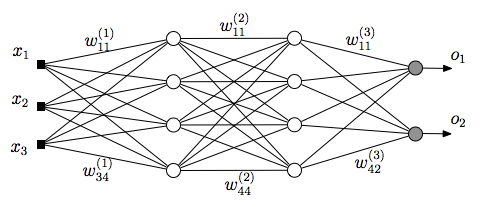
\includegraphics[scale=0.5]{img/MLP}
\caption{Image example}
\label{img:mlp}
\end{figure}


\newpage
\section{\texttt{ALGORITHM\_EXAMPLE} algorithm pseudocode}
\begin{algorithm}[H]
\caption{Algorithm pseudocode example}
\begin{algorithmic}[1]
    \Procedure{ALGORITHM\_EXAMPLE}{$n, d, A$}
    \State $i \gets d $
    \While{$i < n$}
        \ForAll{$r \in A $}
            \State $v \gets f(r)$  \Comment{see fig. \ref{img:mlp}.}
        \EndFor
        \State $i \gets i + 1$
    \EndWhile
\EndProcedure
\end{algorithmic}
\label{alg:multivariate pseudocode}
\end{algorithm}

\end{document}
